\section{The Holy Grail}

\begin{quotex}
All that He wrought among them, all that He said and suffered, He disposed in such wise that not a single moment was passed without mystery, not a single letter was devoid of some mystery. \flright{\textsc{Saint Bernard}, \emph{Sermon III on Palm Sunday}}

In particular, if Christ died on the cross, it can be said that this was by reason of the symbolic value which the cross possesses in itself and which has always been recognized by all traditions; thus, without diminishing in any way its historical significance, the latter may be regarded as directly derived from the symbolical significance that goes with it. \flright{\textsc{Rene Guenon}, \emph{Symbolism of the Cross}}

Since it was the day of Preparation, in order to prevent the bodies from remaining on the cross on the sabbath, the Jews asked Pilate that their legs might be broken, and that they might be taken away. So the soldiers came and broke the legs of the first, and of the other who had been crucified with him; but when they came to Jesus and saw that he was already dead, they did not break his legs. But one of the soldiers pierced his side with a spear, and at once there came out blood and water. \flright{\textsc{John 19:31-34}}

\end{quotex}
There are many legends about the Holy Grail, but there will be no attempt to write a documentary. Instead we will focus on one interpretation in particular, because it reveals the theological and metaphysical significance of the Grail, namely Sergius Bulgakov's essay on the Grail which is an extended meditation on John 19:34.

\paragraph{Primordial Tradition}

The Grail Legend begins with Seth, the third son of Adam and Eve, who was able to rescue the Grail from the Edenic Garden. Then he passed this on so that the Primordial Tradition was never lost to humanity.

The Sufi Suhrawardi also traces it back to Seth (and ultimately to Hermes). He lists Greek philosophers, Persian kings, and Muslim mystics, so the Primordial Tradition was not unknown. Persian sages included the Magi who visited the infant Jesus in Bethelem.

The purpose of the Grail was not fulfilled until it received the Blood and the Water of Christ.

\paragraph{The Death of Christ}
The most common legend is that Joseph of Arimathea captured the blood of Christ in the Grail. Even so, the Cup could not have held all of it, so we can ignore it in Bulgakov's account. Bulgakov points out that Jesus was already dead before the spear was thrust into his side, an anomaly that demands an explanation.

Metaphysically, death is the separation of the soul from the body. Nevertheless, His body did not undergo corruption (Acts 2:31), so there was still a connection of the spirit to the body. Hence, the body was alive although in a state of deep sleep and unconsciousness. This is remarkably close to the definition of the causal body. Since the body was alive, in a sense, the spear caused the blood and water to flow out; Christ's body was then without blood and water.

\paragraph{The Meaning of Blood}
Blood has special significance because it is both material and psychical; thus, it unites the gross body to the animal soul (or life body). The soul, of blood, is intermediate between the body and the spirit. The animal soul lives in the blood; at death, it decays along with the body. The animal soul is not immortal. The human spirit is immortal and animates the soul and indirectly, the body.

Christ's soul was separated from His body after the spear was thrust into his side. The Resurrection restored the soul and blood to the body. That is the blood of the Eucharist. The blood is related in two senses:

\begin{enumerate}
\item The blood is the body of the spirit, the I. 
\item The blood contains the soul of the body 
\end{enumerate}
\paragraph{The Mystery of Golgotha}
Valentin Tomberg, from a different perspective, comes to a similar conclusion:

\begin{quotex}
With the Mystery of Golgotha, when the blood of Jesus Christ flowed onto the ground, a force was planted in human blood and in the Earth's soil; it counteracted the demonic element in the blood and the enslaving influence of the subterranean spheres that works through the soil. This counterinfluence causes human blood to carry not only the subjective illusions of demonic airs, but also the objective impulse of conscience. In addition, this influence not only robs the ground of its enslaving power, but it also speaks of nature's yearning and hope for redemption through humankind. Through it, human blood receives the capacity to reflect moral and spiritual truth, just as natural water reflects the sky; the ground, however, ``receives blood," and thus the capacity of ``groaning together with the whole creation." \flright{\textsc{Valentin Tomberg}, \textit{Christ and Sophia}}

\end{quotex}
\paragraph{The Sanctification of Creation}
The blood and water that flowed from Christ's side into the world, now abides in the world. Bulgakov writes:

Through the stream of Christ's precious blood and water that flowed out of his side, all creation was sanctified—heaven and earth, our earthly world, and all the stellar worlds. The image of the \textbf{Holy Grail} expresses precisely the idea that the world received His holy relic in the blood and water … The whole world is the chalice of the Holy Grail.

That is why it is hidden in the world from the world. There are exceptions:

\begin{quotex}
It exists in the world as an invisible power, and it becomes visible, appears to pure human hearts who are worthy of its appearance.

\end{quotex}
In other words, it does not appear to the gross body but only to the life body (or etheric body), which is why the search continues.

\paragraph{Ascension and Second Coming}
The Ascension into Heaven does not refer to a spatial event. Heaven is not a ``place" somewhere in the cosmos. Rather it indicates a change of state; that is, it refers to the glorification and deification of Christ's human substance. For that reason, it becomes inaccessible to human perception.

That change of state began with the Resurrection when Christ appeared to his disciples. Even after the Ascension, he appeared to Paul. So his abiding in Heaven does not preclude his appearance on Earth.


\begin{wrapfigure}{rt}{.45\textwidth}
 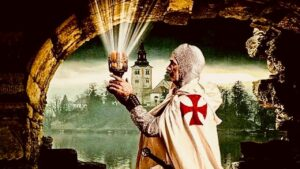
\includegraphics[scale=.5]{a20210403TheHolyGrail-img001.jpg}
\end{wrapfigure}

Likewise, the Second Coming does not refer to a spatial change, the journey from Heaven to Earth. On the contrary, it refers to a change in human beings so that Christ will become visible to those prepared to ``see" him. The Holy Spirit manifests and realizes Christ in them. But first the soul must be purified so that it accurately reflects the Holy Spirit. Then Christ will be born from the union of the Spirit and the body. See The Word is Made Flesh.

\paragraph{The Kingdom of Christ}
The blood and earth restore liberates humanity from its bondage, or at least its possibility. Tomberg explains:

\begin{quotex}
For humanity this influence on blood and earth means the restoration of equilibrium in these regions and hence the establishment of freedom. Now it depends upon human beings themselves whether they will yield to the enslaving influence of earth and the phantasm-producing influence of blood, or whether they will view the whole earthly globe as the victim of the fall of humanity and make blood the bearer of conscience.

\end{quotex}
Bulgakov announces this restoration in the colorful phrase, ``The Great Pan is dead!" By this is meant that the Prince of the World has been cast out of his role and that the World is now the Kingdom of Christ. Even Nature has been changed. The natural world is no longer an obstacle, it is not evil in itself. Rather humanity has been given new powers for the establishment of the Kingdom of God, not only within use, but in the midst of us. A new civilization arises.

Although Satan has been removed as Prince of the World, he still lingers to tempt humanity. Tomberg provides a more complete picture:

\begin{quotex}
The establishment of equilibrium (and with it, human freedom) is not the only result of the Mystery of Golgotha. It was also the beginning of a gradual retrieval of Lucifer's territory. The spirit who had severed this territory from the region of the hierarchies of good now experienced an inner conversion through the Mystery of Golgotha. True, that conversion initially concerned only Lucifer himself and not, say, the Luciferic influence in human beings—which is still active in the old direction and can be changed only by human beings themselves.

\end{quotex}
\paragraph{Redemption}
\begin{quotex}
Most probably we are in Eden still. It is only our eyes that have changed. \flright{\textsc{G K Chesterton}}

\end{quotex}
After the Fall, humanity lost the constant awareness of God (or, lost sanctifying grace); nature fell under the dominion of Satan and was resistant to human effort.

Redemption is the restoration of the status quo ante before the Fall. That means the state in which there is the awareness of God's presence in the life body; nature itself has been changed. But just as the Serpent was in the Garden, Lucifer is still present among us, not as Lord, but as tempter. He has no power over us unless by our consent.

\paragraph{References}
Sergius Bulgakov, \emph{The Holy Grail and the Eucharist}

Valentin Tomberg, \emph{Christ and Sophia}

Sayyed Nasr, \emph{Three Muslim Sages}

Rene Guenon, \emph{Symbolism of the Cross}



\flrightit{Posted on 2021-04-03 by Cologero }

\begin{center}* * *\end{center}

\begin{footnotesize}\begin{sffamily}



\texttt{Paulo Adolpho on 2021-04-05 at 23:47 said: }

Cologero, why god created lucifer, knowing that one day he would turn his back on him. God really likes to see the circus on fire?


\end{sffamily}\end{footnotesize}
